\documentclass[a4paper,14pt]{report}

\usepackage[T2A]{fontenc}
\usepackage[utf8]{inputenc}

\usepackage[english,russian]{babel}

\usepackage{amsthm}

\usepackage{hyperref}

\usepackage[dvips]{graphicx}
\graphicspath{{images/}}

\usepackage{titlesec}
\usepackage{listings}
\usepackage{indentfirst}

\usepackage{geometry}
\geometry{left=3cm}
\geometry{right=1.8cm}
\geometry{top=1.5cm}
\geometry{bottom=2cm}
\renewcommand{\baselinestretch}{1.5}

\lstset{numbers=left,
        frame=single,
        breaklines=true,
        breakatwhitespace=true}
        
%\hyphenpenalty=10000

\begin{document}

\makeatletter
\renewcommand{\@biblabel}[1]{#1.}
\makeatother

\titleformat{\chapter}[hang]{\huge\bfseries}{\thechapter. }{0pt}{\hyphenpenalty=10000\huge\bfseries}

\renewcommand{\theenumi}{\arabic{enumi}}
\renewcommand{\labelenumi}{\arabic{enumi}}
\renewcommand{\theenumii}{.\arabic{enumii}}
\renewcommand{\labelenumii}{\arabic{enumi}.\arabic{enumii}}
\renewcommand{\theenumiii}{.\arabic{enumiii}}
\renewcommand{\labelenumiii}{\arabic{enumi}.\arabic{enumii}.\arabic{enumiii}}

\renewcommand{\lstlistingname}{Листинг}

\newtheorem{Def}{Определение}[section]
\newtheorem{Rule}{Правило}[section]

%\begin{titlepage}
\newpage

\begin{center}
Академия наук и Ко \\
\hrulefill
\end{center}

\vspace{9em}
\begin{center}
Пояснительная записка к дипломному проекту на тему:
\end{center}

\vspace{2.5em}
\begin{center}
\textsc{\textbf{Разработка технологии виртуализации процессоров x86 на arm}}
\end{center}

\vspace{6em}

\begin{flushleft}
Студент \hrulefill Я \\
Научный руководитель \hrulefill Не я \\
\end{flushleft}

\vspace{\fill}

\begin{center}
Не распечатывайте этот титульный лист, он присутсвует только для электронной версии. Возьмите отформатированный титульный лист \href{https://mail.google.com/mail/u/0/?ui=2&ik=92d79e1d27&view=att&th=13e7f4d7588d2a66&attid=0.1&disp=safe&realattid=f_hgf57t580&zw}{здесь}
\end{center}

\end{titlepage}

\chapter{Введение}

\section{Статический анализ кода}

С течением времени программные системы становятся все сложнее. Как следствие, их тестирование занимает все больше времени, при многопоточном программировании особенно часто проявляются ошибки, сложные для обнаружения, воспроизведения и анализа. Вся логика работы программы уже не может быть легко понята и осмысленна одним программистом. В связи с дороговизной ручного тестирования и большой сложностью программынх систем активно развиваются различные виды автоматической проврки программ. Их можно условно разделить на два вида:
\begin{itemize}
\item автоматическая проверка корректности программы во время ее работы или работы ее отдельных частей
\item проверка программы на корректность без ее запуска
\end{itemize}

К первой группе можно отнести всевозможные виды тестирования. 

\begin{Def}\label{static_program_analysis}
Статический анализ кода -- это анализ программного обеспечения, производимый без реального выполнения исследуемых программ.
\end{Def}

Статический анализ позволяет выявить многие виды ошибок еще до запуска программы, большинство из которых сложно искать и воспроизводить непосредственно во время работы приложения. В связи с этим активно развиваются различные инструменты, позволяющие статически доказывать отсутсвие в программах ошибок тех или иных видов.  

\section{Неизменяемость в контексте объектно-ориентированного языка}

В различных контекстах понятие неизменяемости может пониматься по-разному. В данной работе рассмотрено несколько видов неизменяемости:

\begin{Def}\label{immutabule_class}
Неизменяемый класс -- класс, все представители которого являются неизменяемыми. 
\end{Def}

Примером неизменяемого класса является, например, java.lang.String.

\begin{Def}\label{immutable_object}
Неизменяемый объект -- объект, который не может быть изменен, при не гарантируется, что другие представители того же самого класса могут быть изменены.
\end{Def}
Если в какая-либо система позволяет выражать данное свойство объекта, будем говорить, что в данной системе есть поддержка \textit{объектной неизменяемости}.

\begin{Def}\label{reference_immutability}
неизменяемая ссылка -- ссылка, которая не может быть использована для изменения объекта, на который она указывает (при этом объект может быть изменен через другую ссылку).
\end{Def} 

\textit{добавить кратинку}
Если какая-либо система позволяет выражать данное свойство объекта, будем говорить, что в данной системе есть поддержка \textit{ссылочной неизменяемости}. 

Нужно заметить, что данные понятия не являются чем-то искусственным по отношению к языкам программирования. Приведем примеры использования данных понятий в языке программирования Java.

Например, в документации к классу org.joda.time.Period написано: "Неизменяемый временной период..." \footnote{http://joda-time.sourceforge.net/apidocs/org/joda/time/Period.html}. Таким образом, класс org.joda.time.Period является неизменяемым классом. 

\section{Обзор существующих решений}

Рассмотрим, как проблема контроля изменяемости решается в различных объектно-ориентированных языках программирования. 

\subsection{C++}

В языке C++ для выражения неизменяемости используется ключевое слово const. В общем случае можно сказать, что если какое-то значение неизменяемо, то в ту часть памяти компьютера, где оно хранится, не может быть произведена запись. В случае с нессылочными типами данных, если какая-либо переменная объявлена как const, то ее значение не может быть изменено после инициализации. Это означает, что в С++ есть объектная неизменяемость.

\begin{lstlisting}[caption=Константая переменная, label=code:const_var]
struct S
{ 
    int val;
};
 

const S const_s;
const_s.val = 42;      // Error: const_s was declared as const
int i  = const_s.val;  // OK: field val is accessed for reading, 
                           // not for writing

const S non_const_s;
non_const_s.val = 42;  // OK: non_const_s was not declared as const
	

\end{lstlisting}

Для указателей и ссылкок значение модификатора const более сложное. Константным может быть сам указатель, значение, на которое он указывает или оба. Если какая-либо переменная объявлена как константый указатель, то ее значение не может быть изменено после инициализации. Если переменная объявлена как указатель на константный объект, то ее значение может быть изменено, но ее нельзя использовать для изменения объекта, на который она указывает. Таким образом, в C++ есть ссылочная неизменяемость. Нужно заметить, что не существует никакого способа сказать, что некий указатель указывает на неизменяемый объект. Все то же самое касается ссылок. 

\begin{lstlisting}[caption=Константный указатель, label=code:const_pointer]
struct S
{ 
    int val;
};

void Foo( S * ptr,
          S const * ptrToConst,
          S * const constPtr,
          S const * const constPtrToConst )
{
    ptr->val = 0;    // OK: modifies the "pointee" data
    ptr  = NULL;     // OK: modifies the pointer
 
    ptrToConst->val = 0; // Error: cannot modify the "pointee" data
    ptrToConst  = NULL;  // OK: modifies the pointer
 
    constPtr->val = 0; // OK: modifies the "pointee" data
    constPtr  = NULL;  // Error: cannot modify the pointer
 
    constPtrToConst->val = 0; // Error: cannot modify the "pointee" data
    constPtrToConst  = NULL;  // Error: cannot modify the pointer
}
\end{lstlisting}

Методы, которые не изменяют значение объекта, на котором вызываются, могут быть помечены ключевым словом const. Тот факт, что метод действительно не изменяет объект, на котором вызывается, проверяется статически. Методы, помеченные как const могут быть вызваны как на константных, так и на неконстантных объектах. Методы, непомеченные как const, могут быть вызваны только на неконстантных объектах. 

В даном подходе есть несколько недостатков. Первый из них связан с хранением в объекте указателей на другие объекты. Если некий объект является константным, то указатели, хранящиеся в нем в качетсве полей, будут константными, но при этом они могут быть использованы для изменения объекта, на который ссылаются. Рассмотрим пример: 

\begin{lstlisting}[caption=Пример изменения значения по указателю в константном методе, label=code:pointer]
struct S
{ 
    int val;
    int *ptr;
};
 
void Foo(const S & s)
{
    int i  = 42;
    s.val  = i;  // Error: s is const, so val is a const int
    s.ptr  = &i; // Error: s is const, so val is a const int
    *s.ptr = i;  // OK: the data pointed to by ptr is always mutable
}
\end{lstlisting}

Несмотря на то, что s передается в метод Foo() как константый (что также делает константными всех его членов), объект, доступный через s.ptr можно изменять. Таким образом, в C++ нет поддержки глубокой неизменяемости.

Также в С++ невозможно вернуть ссылку, чья изменяемость зависит от изменяемости this. Поэтому, например, во всех колелкциях STL содержатся по две перегруженные версии iterator и operator[], которые, фактически, делают одно и то же, отличаясь только константностью и, как следствие, константностью возвращаемого значения.

\subsection{C\#}

В C\# ключевое слово readonly, примененное к полям имеет слелующий смысл: присвоение значения полю, которое было объявлено с модификатором readonly может произойти либо по месту его объявления, либо в конструкторе, если это нестатическое поле (для статического поля - в статическом конструкторе). 

\begin{lstlisting}[caption=Ключевое слово readonly в C\#, label=code:csharp_readonly]
using System;
public class ReadOnlyTest 
{
   class MyClass 
   {
      public int x;
      public readonly int y = 25; // Initialize a readonly field
      public readonly int z;

      public MyClass() {
         z = 24;   // Initialize a readonly instance field
      }

      public MyClass(int p1, int p2, int p3) {
         x = p1; 
         y = p2;   // OK: readonly field can be reassigned in constructor
         z = p3;
      }
   }

   public static void Main() {        
      MyClass p2 = new MyClass();
      p2.x = 55;   // OK: field x is not readonly
      p2.y = 33;   // Error: field y can't be reassigned, as it is readonly      
   }
}	
\end{lstlisting}

В C\# также есть ключевое слово const, которое обозначает, что значение перменной может быть присвоено только в момент ее объявления. То есть, поля объекта, объявленные как readonly, могут иметь различные значения в зависимости от того, какой конструктор и с какими параметрами был вызван. Поле, объявленное как const всегда будет иметь одно и то же значение.

\begin{lstlisting}[caption=Ключевое слово const в C\#, label=code:csharp_const]
using System;
public class ReadOnlyTest 
{
   class MyClass 
   {
      public int x;
      public const int y = 25; // Initialize a const field

      public MyClass() {
         z = 24;   // Initialize a readonly instance field
      }

      public MyClass(int p1, int p2) {
         x = p1; 
         y = p2;   // Error: const field can not be reassigned in constructor        
      }
   }

   public static void Main() {        
      MyClass p2 = new MyClass();
      p2.x = 55;   // OK: field x is not readonly
      p2.y = 33;   // Error: field y can't be reassigned, as it is const
      
   }
}	
\end{lstlisting}


\subsection{Java}

В языке Java есть ключевое слово final, обозначающее, что значение соответствующего поля или переменной не может быть переприсвоено. Если все поля некоторого объекта объявлены как final, то можно говорить о том, что данный объект неизменяем. Действительно, после завершения конструктора в final поле всегда может находиться один и тот же объект, но сам этот объект может быть изменен. Таким образом, в Java нет поддержки глубокой неизменяемости.

\begin{lstlisting}[caption=Ключевое слово final, label=code:java_final]
public class MyClass {
    public final int[] values;
	
    public MyClass() {
        values = new int[10];    
    }	
}

MyClass mc = new MyClass();
mc.values = new int[100]; // Error: field values was declared final
mc.values[2] = 4; // OK: values is declared final, but we can still
                  // change object, referenced by this field.
    
\end{lstlisting}


Показательным является следующий пример: пусть есть некий класс, который содержит в себе ссылку на список объектов. Разработчик интерфейса этого класса хочет разрешить клиенту получать хранимый список, но не хочет, чтобы клиент мог модифицировать данный список. На Java код такого класса будет скорее всего выглядеть следующим образом:

\begin{lstlisting}[caption=Неизменяемый список, label=code:java_immutable_list]
public class ListContainer {
    private final List<String> values = new ArrayList<String>();   
    
    public List<String> getValues() {
        return Collections.unmodifiableList(values);
    }    
}
\end{lstlisting}

В данном случае, Collections.unmodifiableList(values) вернет обертку над исходным списком, у которой все изменяющие список методы переопределены так, что они бросают UnsupportedOperationException. Основным недостатком данного подхода является то, что ошибка будет обнаружена только во время выполнения программы. Ее локализация и исправление потребуют горадо больше усилий, чем если бы данная ошибка была выявлена на этапе компиляции.

\begin{lstlisting}[caption=Использование неизменяемого списка, label=code:java_immutable_list_usage]
ListContainer container = new ListContainer();
List<String> containerValues = container.getValues();
int size = containerValues.size(); // OK: getting size is permitted for immutable list
containerValues.add("Hello!");     // Error: this code will be successfuly compiled, but 
	                               // will cause UnsupportedOperationException on runtime	
\end{lstlisting}

Таким образом, в стандратной библиотеке Java неизменяемые коллеции реализованы просто как обертки над стандартыми интерфейсами, у которых переопределены изменяющие объект методы. Так как при вызове Collections.unmodifiableList() копирования элементов не происходит, то все изменения, сделанные в исходдной коллекции, будут "видны" в containerValues. Таким образом, результат работы метода ListContainer.getValues() является в некотором смысле неизменяемой ссылкой -- через эту ссылку нельзя менять объект, но существуют другие ссылки на данный объект, через которые его можно менять.

Можно ли каким-либо образом избежать возможной ошибки времени исполнения, при этом не позволяя пользователю добавлять элементы в список values, хранящийся в ListContainer? Можно переписать класс ListContainer следующим образом:

\begin{lstlisting}[caption=Неизменяемый список, label=code:java_immutable_list]
public class ListContainer {
    private final List<String> values = new ArrayList<String>();   
    
    public List<String> getValues() {
        return new ArrayList<String>(values);
    }    
}
\end{lstlisting}

В этом случае, будет создана независимая копия списка values, которая и будет возвращена пользователю. Любые изменения, производимые с этой копией, не затронут исходный список. 

Альтернативный подход можно наблюдать на примере библиотеки gs-collections \footnote{https://github.com/goldmansachs/gs-collections}. В ней есть две отдельные иерархии коллеций -- для изменяемых коллекций и для неизменяемых. Таким образом, попытка вызвать изменяющий коллекцию метод на неизменяемой коллекции приведет к ошибке компиляции.

\begin{lstlisting}[caption=Неизменяемый список, label=code:java_immutable_list]
public class ListContainer{
    private final MutableList<String> values = new FastList<String>();   
    
    public ImmutableList<String> getValues() {
        return values.toImmutable();
    }
    
}
\end{lstlisting}

С одной стороны, этот подход позволяет избежать ошибок, связанных с неправомерным изменением объектов во время выполнения программы, но с дургой его реализация требует написания гораздо большего количества кода. В такоем подходе есть еще одна проблема: структура интерфейсов и их реализации полностью определяются создателем библиотеки и ее пользователь имеет гораздо меньше свободы в ее использовании. 

Часто в документации к Java-коду можно встретить информацию о том, что фактически объект, возвращаемый каким-либо методом является неизменяемым. Или, например, в документации к интрфейсу Map сказано, что "необходима большая осторожность при испрользовании изменяемых объектов в качестве ключей". Наличие подобной информации в документации показывает, что выразительных средств языка не хватает для выражения утвержедний об изменяемости объектов и что, если бы подобные средства существовали, они могли бы быть востребованы.


\subsection{Javari}

Javari -- это расширение языка Java, которое добавляет в Java ссылочную неизменяемость, комбинируя статические и динамические проверки неизменяемости. Авторы вводят следующее определение:

\begin{Def}\label{abstract_state}
Абстрактное состояние объекта -- это состояние самого объекта и все достижимые из него по ссылкам состояния.
\end{Def}

Javari предоставляет гарантии относительно всего транзитивно достижимого состояния объекта -- то есть, состояния самого объекта и состояний всех объектов, доступных из него по нестатическим ссылкам. При этом некоторые части класса могут быть исключены из его абстракного состояния. 

Javari добавляет к Java пять дополнительных ключевых слов assignable, readonly, mutable и romaby. Рассмотрим их использование на примерах.

Пусть, например, переменная rodate имеет тип readonly Date. Тогда rodate не может быть быть использована только для тех операций, которые не меняют объект, на который ссылкается rodate:

\begin{lstlisting}[caption=Неизменяемая ссылка, label=code:readonly_ref]
readonly Date rodate = ...; // readonly reference to a Date object 
rodate.getMonth();    // OK
rodate.setYear(2005); // Error

/*mutable*/ Date date = new Date(); // mutable Date
rodate.getMonth();    // OK
rodate.setYear(2005); // Error
\end{lstlisting}

Пусть в Java существует некий ссылочный типа T. Тогда readonly T в Javari является супертипом T. Изменяемая ссылка может быть использована везде, где ожидатся неизменяемая ссылка. Это связано с тем, что неизменяемая ссылка только лишь запрещает менять объект, на который она ссылается, при этом ничего относительно этого объекта не гарантируя. 

\begin{figure}[h]
\center{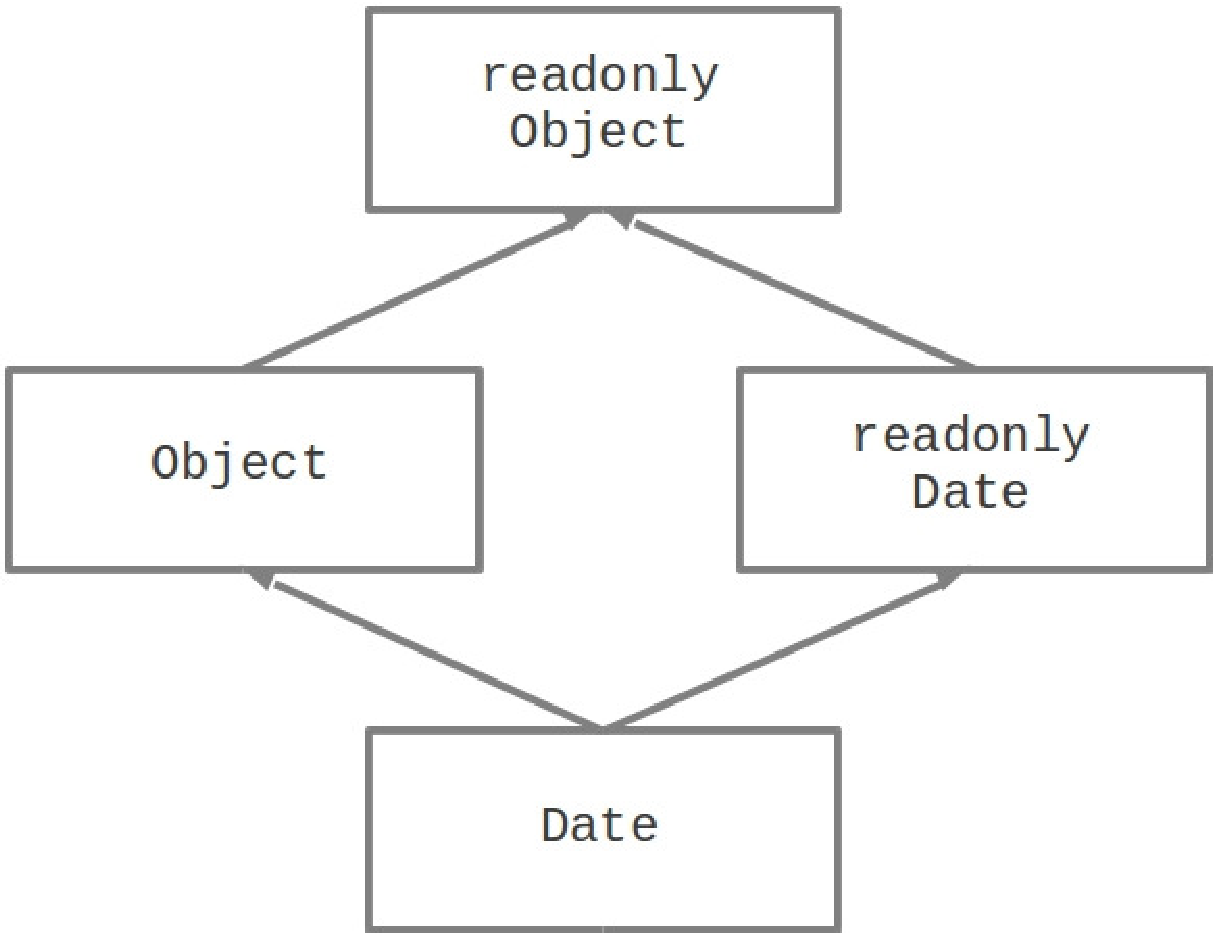
\includegraphics[scale=0.4]{javari_classes.pdf}}
\caption{Фрагмент иерархии классов в Javari}
\label{pic:javari_classes}
\end{figure}

На данном рисунке представлена иерархия типов в Javari. Система типов гарантирует, что изменяющие объект методы не могут быть вызваны на неизменяемых ссылках.

Ключевое слово readonly может быть спользовано при декларации любой переменной, поля, параметра или возвращаемого значения метода. Его также можно применять к неявному параметру this:

\begin{lstlisting}[caption=readonly метод, label=code:readonly_method]
public char charAt(int index) readonly { ... }
\end{lstlisting}

В контексте этого метода this будет неизменяемым.

Модификаторы изменяемости, введенные в Javari не меняют поведения программы во время исполнения. Такой подход обеспечивает обратную совместимость файлов, сгенерированных Javari, с файлами, сгенерированными обычным javac. Одним из последствий такого подходя является то, что два перегруженных метода не могут отличаться только изменяемостью их параметров. Например, такие два метода не могут перегружать друг друга:

\begin{lstlisting}[caption=Перегрузка методов, label=code:javari_method_overloading]
void foo(/*mutable*/ Date d) { ... } 
void foo(readonly Date d) { ... }
\end{lstlisting}

Это аналогично тому, что в Java два перегуженных метода не могут отличаться только типовыми параметрами.

Javari также позволяет исключать некоторые поля из абстрактного состояния объекта. По умолчанию все поля являются частью абстрактного состояния объекта и, соответсвенно, не могу быть изменены через неизменяемую ссылку. Если поле объявлено как assignable, то его значение всегда может быть переприсвоено (даже через read-only ссылку). Ключевое слово mutable означает, что поле может быть изменено даже через неизменяемую ссылку. Это может быть полезно для кэширования данных или, например, для реализации логирования, как в следующем примере:

\begin{lstlisting}[caption=assignable и mutable поля, label=code:assignable_mutable]
class Foo { 
    assignable int hc; 
    final mutable List<String> log = new ArrayList<String>;
    
    int hashCode() readonly { 
        log.add("hashCode invoked");
        if (hc == 0) { 
            hc = ... ;
        } 
        return hc; 
    } 
}
\end{lstlisting}

Javari также позволяет добавлять модификаторы изменяемости к типовым параметрам:

\begin{lstlisting}[caption=Модификаторы изменяемости в типовых параметрах, label=code:javari_generic_local]
/*mutable*/ List</*mutable*/ Date> ld1; // add/remove and mutate elements 
/*mutable*/ List<readonly Date> ld2; // add/remove 
readonly List</*mutable*/ Date> ld3; // mutate elements 
readonly List<readonly Date> ld4; // (neither)
\end{lstlisting} 

Можно представить себе ситуацию, когда программисту захочется управлять изменяемостью типового параметра: например, написать mutable X, где X -- типовый параметр:

\begin{lstlisting}[caption=Модификаторы изменяемости и типовые параметры, label=code:javari_generic_mutable]
class Container<X> {
    void foo() {
       mutable X x = ...;
    }
}
\end{lstlisting} 

Javari запрещает такие типы потому что это не сочетается с подходом к типовым параметрам, принятым в Java, и это может привести к превращении неизменяемой ссылки в изменяемую. Но в Javari, как и в Java, автор класса с типовым параметром может наложить на этот параметр границы. В примере ниже параметр X модет быть readonly Date, mutable Date или каким-либо из их наследников, в то время как Y может быть только mutable Date или его наследником. 

\begin{lstlisting}[caption=Объявление класса с типовыми параметрами, label=code:javari_generic_class]
class Foo<X extends readonly Date, Y extends mutable Date> { ... }
\end{lstlisting} 

Также Javari позволяет абстрагироваться от изменяемости типового параметра. Это можно сделать с помощью конструкции ? readonly C, где С -- какой-то тип. Так, List<? readonly Date> является суперклассом для List<readonly Date> и List<mutable Date>. 

\begin{figure}[h]
\center{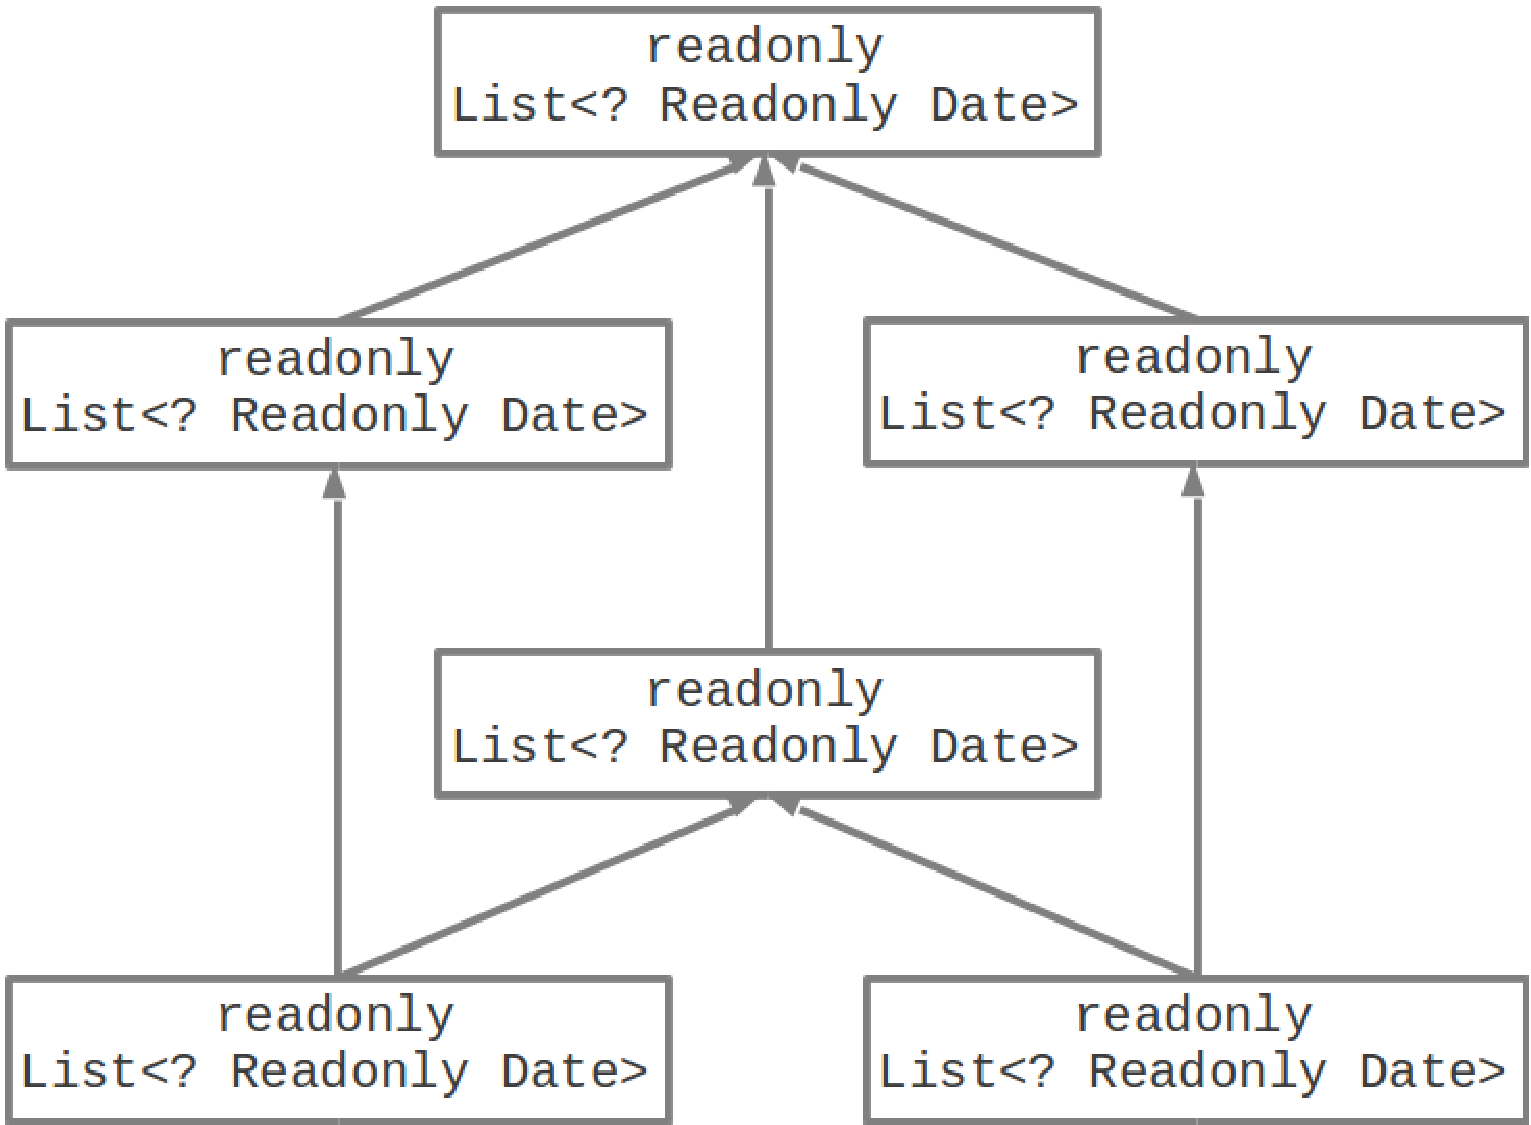
\includegraphics[scale=0.4]{javari_list_classes.pdf}}
\caption{Фрагмент иерархии классов в Javari}
\label{pic:javari_list_classes}
\end{figure}


Наконец, рассмотрим назначение ключевого слова romaybe. Пусть есть класс DateCell, который хранит в себе значение типа Date. Необходимо определить метод getValue, который будет возвращать это значение. Какого модификатор изменяемости должен стоять на возвращаемом значении? Если метод getValue вызывается на изменяемом объекте, то и его результат должен быть изменяемым. Если же он вызван на неизменяемом объекте, и результат его выполнения должен быть неизменяемым. Для решения этой проблемы в Javari было введено еще одно ключевое слово - romaybe. Так будет выглядеть класс DateCell с использованием этого ключевого слова:

\begin{lstlisting}[caption=Ключевое слово romaybe, label=code:javari_romaybe]
class DateCell { Date value; romaybe Date getValue() romaybe { return value; }
}
\end{lstlisting}

В данной ситуации для системы типов существует два метода getValue: в первом все ключевые слова romaybe будут заменены на readonly, а во втором просто опущены. 

Javari предоставляет инструмент под названием Javarifier, позволяющий добавить модификаторы изменяемости к уже существующему коду. На входе он принимает класс-файлы. В начале работы алгоритма некоторые поля помечаются как assignable или mutable (например, на основании того, что они меняются в методе hashCode). Данный алгоритм генерирует и решает систму утверждений для анализируемой программы. Используются два типа утверждений:
\begin{itemize}
	
	\item \textit{некотнтролируемое утверждение} о том, что некая ссылка является неизменяемой: "x is mutable"
	
	\item \textit{контролируемое утверждение} о том, что некая ссылка явлется измеянемой, если другая ссылка является изменяемой: "if y is mutable then x is mutable"
	
\end{itemize}
После составления системы утверждений алгоритм рашает ее.

Минусом данного подхода является то, что в общем случае количество уравнений а данной системе $~O(n^2)$, где n - количесвто ссылок в анализируемом коде. 

\subsection{Immutability Generic Java}

Immutablility Generic Java (IGJ) -- это расширение языка Java, которое позволяет выражать утверждения о неизменяемости объектов без внесения изменений в синтаксис Java, для этого IGJ использует типовые параеметры и аннотации. В IGJ каждый класс имеет дополнительный типовый параметр, который может быть Immutable, Mutable или ReadOnly. IGJ поддерживает как объектную так и ссылочную неизменяемость. IGJ также разрешает ковариантные изменения типовых параметров в безопасной форме, например, неизменяемый список целых чисел является потомком неизменяемого списка чисел.

Рассмотрим применение данного расширения на примере:

\begin{lstlisting}[caption=Ключевое слово romaybe, label=code:igj_graph]
class Edge<I extends ReadOnly> {
    private long id;
    
    @AssignsField Edge(long id) {
        this.setId(id);
    }
    
    @AssignsField synchronized void setId(long id) {
        this.id = id;
    }
    
    @ReadOnly syncronized long getId() {
        return id;
    }
    
    @Immutable long getIdImmutable() {
        return id;
    }
    
    @ReadOnly Edge<I> copy() {
        return new Edge<I>(id);
    }
    
    static void print(Edge<ReadOnly> e) {...}
}

class Graph<I extends ReadOnly> {
    List<I, Edge<I>> edges;
    
    @AssignsField Graph(List<I, Edge<I>> edges) {
        this.edges = edges;
    }
    
    @Mutable void addEdge(Egde<Mutable> e) {
        this.edges.add(e);
    }
    
    static <X extends ReadOnly> Edge<X> 
        findEdge(Graph<X> g, long id) {...}
}
\end{lstlisting}

В примере \ref{code:igj_graph} представлены два IGJ сласса: Edge и Graph. В строчках 1 и 27 определен параметр неизменяемости I. Если в декларации класса отсутсвует дирректива extends, считается, что класс наследует Object<I>. Присваивание this.id = id разрешено, так как метод setId помечен как Mutbale. Метод print, например, принимает любой объект типа Egde, вне зависисмости от его изменяемости. Одним из плюсов IGJ является то, что тот факт, что поля некотго объекта имеют тот же параметр изменяемости, что и сам объект, легко выражается при помощи типовых параметров, как, например это сделано в строке 28. Например, в С++ поля, не обозначенные как const или mutable имеют модификатор неизменяемости такой же, как и у объекта, их содержащего, но при этом отсутсвует возможность указать, что какая-либо локальная переменная, параметр метода или возвращаемое значение имеют такую же неизменяемость, как и объект, на котором данный метод вызван, IGJ же предоставляет такую возможность.

Аннотация @AssignsField решает проблему с изменяемостью this в конструкторе. В контсрукторе неизменяемого объекта нельзя счиать this Mutable, так как в этом случае такая изменяемая ссылка могла бы "утечь". Из метода, проаннотированного как AssignsField ссылка на this может "утечь" только как ReadOnly ссылка. 

Подход, описанный в данной работе, несомненно, позволяет выражать различные утверждения о неизменяемости объектов. Но у него есть несколько минусов:
\begin{itemize}
\item Получающийся код часто выглядит достаточно громоздко.
\item Фаза конструирования объекта заканчивается тогда, когда заканчивает работу его конструктор. Это не позволяет достаточно легко создавать неизменяемые циклические структуры данных. Существующее расширение OIGJ \textit{ссфлка на работу} решает проблему с конструированием объектов, но делает это путем введения понятия владения объектом и, как следствие, добавлением еще одного типового параметра к каждому типу. 
\item Для того, чтобы эффективно использовать уже существующий код из классов, написанных с использованием IGJ необходимо вручную добавить в него дополнительные типовые параметры, отвечающие за изменяемость обхектов
\end{itemize}

\subsection{D}

Подход, похожий на тот, что был описан в IGJ используется в объекно-ориентированном языке D~\footnote{http://dlang.org/}. В D концепции объектной и ссылочной неизменяемости поддерживаются на уровне языка.

Во второй версии этого языка существует два ключевых слова для выражения неизменяемости: const и immutable. Ключевое слово immutable означает, что не существует ссылки, через которую данные могут быть изменены. const обозначает, что по данной ссылке данные менять нельзя, но может существовать ссылка, через которую данные могут быть изменены. 

\begin{lstlisting}[caption=const vs immutable, label=code:d_const_vs_immutable]
int[] foo = new int[5];     // foo is mutable.
const int[] bar = foo;      // bar is a const view of mutable data.
immutable int[] baz = foo;  // Error:  all views of immutable data must be immutable.
 
immutable int[] nums = new immutable(int)[5];  // No mutable reference to nums may be created.
const int[] constNums = nums;                  // Immutable is implicitly convertible to const.
int[] mutableNums = nums;                      // Error:  Cannot create a mutable view of immutable data.
\end{lstlisting}

В отличае от const в C++, const и immutable в D обеспечивают полноценную глубокую неизменяемость, то есть, любые данные, доступные через const или immutbale объект, также константны или неизменяемы, соответсвенно.

\begin{lstlisting}[caption=const vs immutable, label=code:d_const_vs_immutable]
class Foo {
    Foo next;
    int num;
}
 
immutable Foo foo = new immutable(Foo);
foo.next.num = 5;  // Error:  foo.next is of type immutable(Foo).
                   // foo.next.num is of type immutable(int).
\end{lstlisting}

\subsection{Uniqueness and Reference Immutability for Safe Parallelism}

В работе Uniqueness and Reference Immutability for Safe Parallelism представлено расширение для языка C\#. Основной задачей этого расширения является ограничение изменений областей памяти при параллельном программировании. Это достигается компбинацией модификаторов изменяемости и уникальности. Система типов поддерживает полиморфизм относительно этих модификаторов, а также простое создание циклов неизменяемых объектов.

В рамках данной работы у каждой сслки может быть один из следующих модификаторов:
\begin{itemize}
\item writable -- "обычная" ссылка, позволябщая изменять объект, на который она ссылается
\item readable -- неизменяемая ссылка, которая не позволяет изменять объект, на который она ссылается
\item immutbale -- ссылка на неизменяемый объект
\item isolated -- уникальная ссылка на кластер объектов (то есть, все пути в этот подраф объектов извне будут идти через эту ссылку)
\end{itemize}

Введение такого понятия, как isolated ссылка, повзоляет решить проблему с созданием неизменяемых циклических структур данных, так как если некая ссылка явлется едиснвтенной ссылкой на некий подграф объектов, то изменяемость этого подграфа может быть едитновременно безопасно изменена, так как не существует других ссылок на данный подграф. 

В предложенном в данной работе языке отсутсвуют глобальные изменяемые переменные и поля, исключаемые из состояния объекта, что позволяет, напрмиер, говорить о том, что через readable ссылку не может быть достигнута никакая writable ссылка. Подобные ограничения полезны при анализе многопоточного поведения программы, но для статического контроля за изменяемостью они представляются слишком сильными. Например, введение подобный ограничений для Java означало бы отказ от не-final статических полей, а так же от хранения в статических полях объектов, чье стостояние может быть изменено. Также в данной работе никак не рассмотрен вопрос о том, каким образом при наличии всех этих ограниченйи могу бы быть использован уже существующий код.






























\section{Постановка задачи}

Целью данной работы была разработка системы, позволяющей контролировать изменяемость объектов на этапе компиляции для языка Java. 

К данной системе были предъявлены следующие требования:

\begin{itemize}
	\item Должна быть поддержана как объектная, так и ссылочная неизменяемость.
	
	\item Негобходима возможность исключать некоторые поля из абстрактного состояния объекта. 
	
	\item Данная система должна давать возможность создавать неизменяемые циклические структуры объектов.
	
	\item Необходимо иметь вохможность использовать уже существующий код.
\end{itemize}

В рамках данной работы решались следующие задачи:

\begin{itemize}

	\item Разработка системы аннотаций, позволяющей выражать неизменяемость объектов.
	
	\item Разработка алгоритма вывода аннотаций для существующего кода.

\end{itemize}




\chapter{Статический контроль за изменяемостью объектов}

\section{Подход к технической реализации}

Предположим, нужно добавить некоторую новую функциональность в язык программирования. Есть два принципиально разных способа это сделать:
\begin{itemize}
	\item использовать существующие средства языка
	\item изменять синтаксис языка (например, добавить новые ключевые слова)
\end{itemize}

У обоих этих подходов есть как положительные, так и отрицательные стороны. Изменение синтаксиса языка приводит к невозможности использования многих существующих инструментов для разработки с использованием этого языка, таких как компиляторы, среды разработки, различные анализаторы кода. Но с другой стороны этот подход позволяет добавлять в язык развитую систему выразительных средств. Использование же существующих средств языка ограничивает свободу введения новых концепций, но этот подход обычно гораздо проще в реализации и не влияет на используемые инструменты.

В случае Java есть несколько способов добавить поддержку неизменяемости объектов в язык. В работе IGJ это сделано с помощью добавления дополнительного типового параметра ко всем классам. Но это выглядит очень громоздко и трудно читаемо. Другой варинат -- использование аннотаций. 

Аннотация в Java -- это вид метаданных, которые могут быть добавлены в исходный код. Они могут быть доступны на этапе компилляции, в класс-файлах, а также могут использоваться JVM во время исполнения программы. В Java 7 аннотации можно применять к пакетам, классам, методам, переменным и параметрам. 

Как справедливо отмечают некоторые авторы, аннотации в том виде, в котором они реализованы в Java 7, не достаточно мощны для того, чтобы добавить поддержку контроля за изменяемостью объектов, так как в нынешней реализации нельзя аннотировать типы. Но уже в Java 8 такая поддержка появится, поэтому в данной работе именно аннотации используются для выражения неизменяемости объектов.

\section{Система аннотаций}

Будем считать, что каждая ссылка имеет модификатор изменяемости, который определяет, может ли быть изменено абстрактное состояние объекта, на который она ссылается. Этот моификатор определяется на уровне исходного кода, анализуруется на этапе компиляции и может иметь одно из четырех значений: Mutable, Immutable, ReadOnly или Isolated. На изображении ниже представлена иерархия параметров неизменяемости. 

\begin{figure}[h]
\center{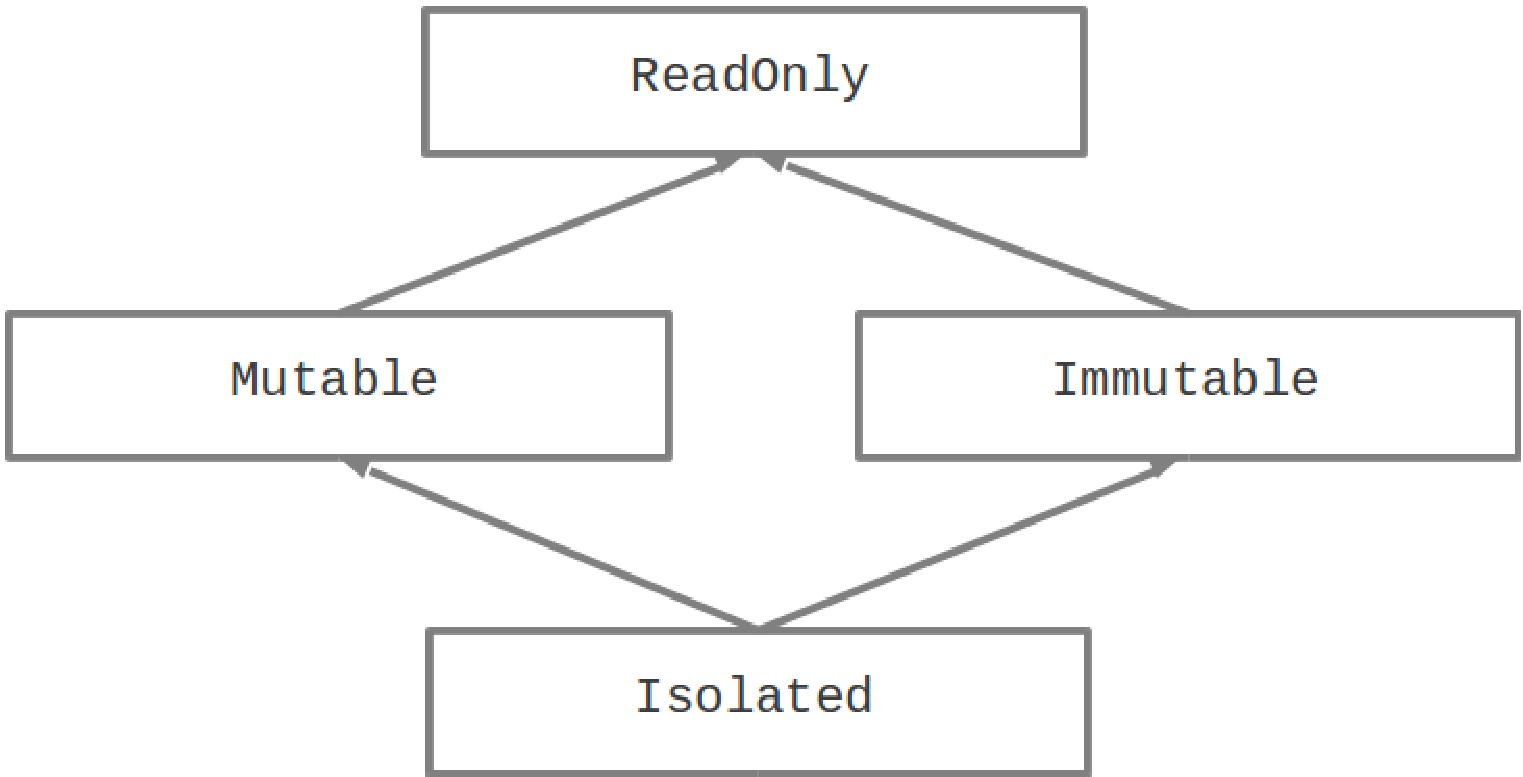
\includegraphics[scale=0.4]{my_classes.pdf}}
\caption{Иерархия модификаторов неизменяемости}
\label{pic:my_classes}
\end{figure}

Выражение $A \preceq B$ будем тракторвать как "$A$ является наследником $В$". В данном случае, например, $Mutable \preceq ReadOnly$. Также будем считать, что если $A \preceq B$, где $А$ и $B$ - модификаторы изменяемости, то $@A\:С \preceq @B\:C$, где $С$ - некий тип.

\subsection{Ссылочная неизменяемость}

Для поддержки ссылочной неизменяемости достаточно двух модификаторов: Mutable и ReadOnly. Состояние объекта не может быть изменено через ReadOnly ссылку. Попытка присвоить поле через ReadOnly ссылку или вызвать на ней меняющий объект метод приведет к ошибке компиляции:

\begin{lstlisting}[caption=Mutable и RadOnly ссылки, label=code:mutable_vs_readonly]
@ReadOnly Person roPerson = ...;
String address = roPerson.address; // OK: reading field is 
                                   // always permitted
roPreson.address = "new address"; // Error: field can't be 
                                  // assigned through ReadOnly referernce

@Mutable Person mPreson = ...;
mPerson.address = "new address"; // OK: mPerson is mutable, 
                                 // so field can be assigned
\end{lstlisting} 

Пусть I(x) - это функция, которая принимает класс, тип или ссылку и возвращает ее модификатор изменяемости. Тогда вышеизложенное правило может быть написано следующим образом:

\begin{Rule}\label{rule:assign_field}
o.someField = ... разрешено тогда и только тогда, когда $I(o) = Mutable$ 
\end{Rule}

Изменяемая ссылка может быть передана везде, где ожидается неизменяемая ссылка. Таким образом, @Mutable Person является наследником @ReadOnly Person.

\subsection{Аннотации на методах}

В Java ключевое слово this внутри конструктора или нестатического метода является ссылкой на текущий объект.  Изменяемость this зависит от контекста, а именно от метода, в котором появляется this. По умолчанию все методы изменяют объект, на котором вызываются. В таких методах this будет иметь модификатор Mutable. Те методы, которые не изменяют объект, на котором они вызываются, должны быть помечены аннотацией @Const (по аналогии с C++), this в этих методах будет иметь модификатор @ReadOnly.

На ReadOnly ссылках нельзя вызывать методы, которые меняют объект, на котором вызываются. Формально это правило может быть описано так:

\begin{Rule}\label{rule:invoke_method}
o.m(...) разрешено, если $I(o) \preceq I(m)$, где I(m) -- модификатор изменяемости this в этом методе.
\end{Rule}

Требуется, что $I(o) \preceq I(m)$ а не $I(o) = I(m)$ для того, чтобы через изменяемую ссылку можно было вызывать методы, не меняющие объект. 

Рассмотрим на примере применение этих правил.

\begin{lstlisting}[caption=Аннотации на методах, label=code:method_annotations]
class Person {
    String name;
    @AsClass Date dateOfBirth;	
    
    public Person(String name, Date dateOfBirth) {
    	this.name = name;
    	this.dateOfBirth = dateOfBirth;
    }
    
    public void setName(String name) {
        this.name = name;
    }
    
    @Const
    public String getName() {
        return name;
    }
    
    @AsClass
    @Const
    public Date getDateOfBirth() {
        return dateOfBirth;
    }
    
    @Const 
    public boolean wasBornInYear(int year) {
    	return dateOfBirth.getYear() == year;
    }
    
    public void setYearOfBirth(int year) {
        dateOfBirth.setYear(year);
    }
    
    public static void print(@ReadOnly Person person) {
        ...
    }
}
\end{lstlisting} 

Присваивание this.name = name в 11 строке разрешено, так как $I(this) = I(setName) = Mutable$, а согласно правилу \ref{rule:assign_field} через Mutable ссылку можно присваивать значение поля. Это присваивание было бы не разрешено, если бы оно было перемещено  на 16 строку, так как this является ReadOnly ссылкой в контексте метода getName. Вызов метода setYear на 31 строке разрешен согласно правилу \ref{rule:invoke_method}, так как $I(dateOfBirth) = I(this) \preceq I(setyearOfBirth)$. Этот вызов метода не был бы разрешен на 27 строке, так как в контексте метода wasBornInYear $I(this) = ReadOnly$. Статический метод print на 34 строке принимает объект класса Person с любым модификатором изменяемости. 

Поле dateOfBirth проаннотировано @AsClass. Это значит, что его модификатор изменяемости зависит от того, какой модификатор у this. Соответсвенно и результатом работы метода getDateOfBirth будет либо Mutable ссылка (если сам он был вызван на объекте, доступном по Mutable ссылке), либо ReadOnly ссылка в противном случае:

\begin{lstlisting}[caption=Использование аннотации AsClass, label=code:as_class]
@ReadOnly Person roPerson = ...;
// OK: I(getYear) = ReadOnly
int year = roPerson.getDateOfBirth().getYear(); 
// OK: I(roPerson.getDateOfBirth()) = I(roPerson) = ReadOnly
roPerson.getDateOfBirth().setYear(2000); 
	
@Mutable Person mPerson = ...;
// OK: I(mPerson.getDateOfBirth()) = I(mPerson) = Mutable
mPerson.getDateOfBirth().setYear(2000); 
}
\end{lstlisting} 

Аннотация AsClass может встречаться на полях метода, локальных переменных, возвращаемых значениях нестатических методов и параметрах методов.

\subsection{Перегрузка методов}

При перегрузке методов, метод класса-потомка должен оставить прежним или усилить модификатор неизменяемости, который имеет this в данном методе. 

\begin{Rule}\label{rule:override_method}
Если метод $m'$ перегружет метод m, то $I(m) \preceq I(m')$
\end{Rule}

Например, метод класса-потомка может добавить аннотацию Const к перегружаемому методу, если ее не было в классе-предке, но не наоборот. 

\subsection{Объектная неизменяемость}

Хотя ReadOnly ссылки запрещают менять объект, на который ссылаются, никто не гарантирует, что этот объект не будет изменен при помощи какой-либо другой ссылки. Это хорошо иллюстрирует слудющий пример:

\begin{lstlisting}[caption=Изменение объекта\, хранимого по ReadOnly ссылке, label=code:change_ro_object]
@Mutable Person person = ...;
person.setYearOfBirth(2000);
@ReadOnly Person roPerson = person; // OK: @ReadOnly Person is 
                                    // supertype for @Mutable person
// 2000 will be printed
System.out.println(roPerson.getyearOfBirth());
person.setyearOfBirth(2013);
// 2013 will be printed
System.out.println(roPerson.getyearOfBirth()); 			
}
\end{lstlisting} 

При этом часто возникает ситуация, когда хочется не только гарантировать, что по данной ссылке нельзя менять объект, но и то, что данный объект вообще нельзя менять. Такие гарантии могут быть полезны, например, при многопоточном программировании -- если про объект известно, что он неизменяемый, то к нему можно безопасно обращаться из нескольких потоков без дополнительной синхронизации. Разработанная в данной работе система может давать такую гарантию: Immutable ссылка всегда указывает на неизменяемый объект. 

\begin{lstlisting}[caption=Mutable и Immutable ссылки, label=code:mutable_vs_immutable]
@Mutable Person person = ...;
@Immutable Person iPerson = person; // Error: @Immutable Person is 
                                    // not supertype for @Mutable Person
@ReadOnly Person roPerson = iPerson; // OK: @ReadOnly Person is 
                                     // supertype for @Immutable Person
}
\end{lstlisting} 

Из данного примера видна разница между ReadOnly и Immutable ссылками: если ReadOnly ссылка может указывать как на изменяемый, так и на неизменяемый объект, то Immutable ссылка всегда указывает только на неизменяемый объект.  

\subsection{Исключение полей из абстрактного состояния объекта}

Одной из целей данной работы была разработка системы типов, которая бы давала гарантии относительно абстрактного состояния объектов, а не конкретной его реализации. Транзитивные гарантии неизменяемости для всех полей объекта в некоторых случаях могут быть слишком сильны. Например, поля, используемые для кэширования, часто не являются частью абстрактного состояния. Таким образом, необходим механизм, позволяющий исключать некоторые поля из абстрактного состояния объекта. В данной работе для этого используется аннотация @Transient, которая обозначает, что данное поле не является частью абстрактного состояния. 

Многие авторы (\cite{Zibin2007}, \cite{Tschantz2006}) разделяют два способа исключения поля из абстрактного состояния:
\begin{itemize}
\item{Значение поля может быть переприсвоено даже через неизменяемую ссылку, но само значение в этом случае не может быть изменено}
\item{Значение поля не может быть переприсвоено, но при этом значение поля может быть изменено даже через ReadOnly ссыллку}
\end{itemize}
Этот подход кажется несколько избыточным: такая тонкая настройка изменяемости нужна крайне редко и при этом приводит к некоторым проблемам в системе типов, которые приходится решать введением новых правил. Мы используем слеудющее правило: если поле помечено как @Transient, то его значение может быть присвоено вне зависимости от изменяемости объекта, при этом изменяемость самого значения регулируется дополнительной аннотацией (@ReadOnly, @Immutable или @Mutable).

\subsection{Вложенные классы}

Статические вложенные классы подчиняются всем тем же правилам, что и обычные классы. Нестатические вложенные классы имеют дополнительную ссылку на this. Изменяемость this зависит от того, в каком методе он вызван. Метод нестатического вложенного класса может быть объявлен как Const только если он не меняет обе ссылки this (свою и внешнего класса). Для неизменяемого объекта могут быть созданы только неизменяемые экземпляры его вложенных классов. 

\subsection{Неизменяемые классы}

Существуют классы, все представители которых являются неизменяемыми объектами. Таковыми являются, например, java.lang.String и большинство потомков java.lang.Number. Обычно тот факт, что все представители некоего класса являются неизменяемыми, отражается в документации. Для этого разрешено использовать аннотацию @Immutable. Все методы класса, объявленного как Immutable будут обрабатываться так, как будто они аннотированы как @Const.

\subsection{Создание циклов неизменяемых объектов}

Большинсвто неизменяемых объектов, тем не менее, модифицируются во время фазы их конструирования. Например, в неизменяемый список нужно сначала добавить все элементы. В этот момент список фактически будет меняться. Часто эта фаза локализуема непостредственно в конструкторе объекта -- например, в конструктор неизменяемого списка может быть передан набор объектов, которыми этот список нужно заполнить, и после завершения конструктора объект уже можно по праву считать неизменяемым. Несмотря на то, что для большинства объектов фаза их создания заканчивается посе отработки конструктора, бывают случаи, когда такой подход неприменим. Одним из наиболее ярких примеров этого могут служить неизменяемые циклические структуры данных. Рассмотрим следующий пример:

\begin{lstlisting}[caption=DoubleLinkedListNode.java, label=code:circular_list_node]
class DoubleLinkedListNode {
    @AsClass DoubleLinkedListNode prev;
    @AsClass DoubleLinkedListNode next;
    
    @Immutable
    public static DoubleLinkedListNode createTwoNodeList() {
    	// ???
    }
}
\end{lstlisting} 

Необходимо реализовать метод createTwoNodeList, который вернет неизменяемый двусвязный список из двух элементов. Это сделать не получится, так как соединять элементы списка друг с другом придется уже после создания. Можно, конечно, возвращать не Immutable ссылку, а ReadOnly:
 
\begin{lstlisting}[caption=DoubleLinkedListNode.java, label=code:circular_list_node_ro]
class DoubleLinkedListNode {
    @AsClass DoubleLinkedListNode prev;
    @AsClass DoubleLinkedListNode next;
    
    @ReadOnly
    public static DoubleLinkedListNode createTwoNodeList() {
    	@Mutable DoubleLinkedListNode n1 = 
                               new DoubleLinkedListNode();
        @Mutable DoubleLinkedListNode n2 = 
                               new DoubleLinkedListNode();
    	
        n1.next = n2;
        n2.prev = n1;
    
        return n1;  
    }
}
\end{lstlisting} 

Нетрудно видеть, что этом случае созданный список фактически будет неизменяемым, так как после завершения этапа создания, на него не останется ни одной Mutable ссылки. Но этот момент необходимо было бы дополнительно отражать в документации, также результат работы этого метода не мог бы быть использован для передачи в метод, который требует именно Immutable ссылку. 

Ключевым моментом в объяснении того, почему именно результатом работы метода createTwoNodeList будет неизмяенемый объект было следующее утверждение: \textit{после завершения этапа создания, на него не останется ни одной Mutable ссылки}. На самом деле, важно еще и то, что Mutable ссылок не осталось и на другие транзитивно-достижимые из данного объекта объекты. И так как в данном случае это утверждение верно, то объект фактически является неизменяемым. Таким образом, можно прийти к определению \textit{изолированной ссылки}:

\begin{Def}\label{isolated_ref}
Изолированная ссылка (Isolated) -- это ссылка на изолированный граф объектов. Объекты внутри изолиованного графа могут ссылаться друг на драга, но существует только одна внешняя не-ReadOnly ссылка на такой граф. Все пути к не Immutable объектам, доступным через Isolated ссылку, идут через это ссылку кроме путей, идущих по ReadOnly ссылкам.
\end{Def}

Изолированная ссылка может быть единовременно конвертирована в Mutable или Immutable ссылку, так как на граф объектов, достижимых через нее, есть только ReadOnly ссылки, которые не гарантируют ничего относительно этого графа. 

Превращение Isolated ссылки в Mutable ссылку происходит тривиальным образом:

\begin{lstlisting}[caption=Превращение Isolated ссылки в Mutable, label=code:isolated_to_mutable]
@Isolated Person p = ...;
p.setName("Bob");
\end{lstlisting} 

Здесь в строке 2 происходит неявное преобразование модификатора изменяемости p в Mutable.

Isolated ссылка может быть также единовременно сконвертирована в Immutable ссылку.

\begin{lstlisting}[caption=Превращение Isolated ссылки в immutable, label=code:isolated_to_immutable]
@Isolated Person p = ...;
@Immutable imp = p;
p.setName("Alice"); // Error
\end{lstlisting} 

Не смотря на то, что p была изначально объявлена как Isolated, после присовения в imp она была приведена к Immutable и объект, на который она ссылается, не может быть изменен.

Важный момент заключается в том, что превращение Isolated ссылки в Mutable не является необратимым. Например, следующий пример не содержит ошибок компиляции:

\begin{lstlisting}[caption=Превращение Isolated ссылки в Mutable и обратно, label=code:isolated_to_mutable_and_back]
@Isolated
public IntBox increment(Isolated IntBox b) { 
    b.value++; 
    return b;
}
\end{lstlisting}

В данном случае превращение ссылки обратно в Isolated возможно, так как фактически ссылка b осталась изолированной. В работе \cite{Gordon2012} было сформулировано следующее правило, которое обуславливает, может ли Mutable ссылка быть превращена обратно в Isolated после выполнения некой операции:

\begin{Rule}\label{rule:convert_isolated}
Если входной контекст выражения не содержит Mutable ссылок, а выходной контекст выражения содержит одну Mutable ссылку, то эта ссылка может быть превращена обратно в Isolated.
\end{Rule}

Действительно, в случае, когда язык запрещает иметь глобальные изменяемые значения, а также исключать поля из абстрактого состояния объекта, это правило работает. Если после проведения какой-либо операции появилась одна Mutable ссылка, а перед началом операции ни одной Mutable ссылки не существовало, то эта ссылка либо является ссылкой на объект, на который других ссылок не существует, либо на объект, который был только что создан. 

Но запрет на существование глобальных изменяемых переменных является слишком сильным ограничением, так как в существующем коде уже имеется большое количесвто подобных примеров. При этом очевидно, что существуют методы, которые никаким образом не взаимодействуют с глобальными изменяемыми переменными и полями, которые исключены из абстрактного состояния объекта. Будем называть такие методы чистыми и аннотировать их как @Pure. Тогда вышеприведенное правило применимо в контексте Pure метода. Остальные типовые правила для Isolated ссылок будут аналогичны тем, что приведены в \cite{Gordon2012}.

Рассмотрим, каким образом введение Isolated ссылок может решить проблему с созданием циклов неизменяемых объектов:

\begin{lstlisting}[caption=DoubleLinkedListNode.java, label=code:circular_list_node_isolated]
class DoubleLinkedListNode {
    @AsClass DoubleLinkedListNode prev;
    @AsClass DoubleLinkedListNode next;
    
    @Mutable
    @Pure
    private static CircularListNode doCreateTwoNodeList() {
    	@Mutable DoubleLinkedListNode n1 = 
                                 new DoubleLinkedListNode();
        @Mutable DoubleLinkedListNode n2 = 
                                 new DoubleLinkedListNode();
    	
        n1.next = n2;
        n2.prev = n1;
    
        return n1;  
    }
    
    @Immutable
    public DoubleLinkedListNode createTwoNodeList() {
        @Isolated DoubleLinkedListNode result = 
                                 doCreateTwoListNode();
        return result;
    }
}
\end{lstlisting} 

\section{Алгоритм вывода аннотаций}

При разработке реальных приложений обычно используется большое количество библиотечного кода. Проаннотировать весь этот код вручную аннотациями неизменяемости не представляется возможным. Чтобы предложенную нами систему аннотаций можно было использовать в реальных приложениях, нужно обеспечить возможность работать с непроаннотированным кодом. Самое простое решение -- это объявить, что все методы меняют объекты, на которых вызываются. Но тогда практически все объекты во вновь написанном коде (уже с использованием модификаторов неизменяемости) окажутся Mutable. 

Таким образом, необходимо разработать способ проаннотировать существующий код в автоматическом режиме. Далее представлено описание алгоритма, который позволяет вывести соответсвующие аннотации по байткоду. 

Пусть необходимо проаннотировать байт-код некой библиотеки. При этом, возможно, аннотации на некоторых методах или их параметрах уже известны (например, в документации явно написано, что все экземпляры некого класса являются неизменяемыми). Считается, что эти наперед данные аннотации проставлены правильно. Далее рассмотрены этапы аннотирования кода этой библиотеки.

\subsection{Поля, не входящие в абстрактное состояние объекта}

На первом этапе анализа все поля, объявленные как transient помечаются аннотацией @Transient. Все остальные поля помечаются как @AsClass. 

\subsection{Анализ методов на чистоту}

На этом этапе необходимо проставить аннотации @Pure на тех методах, которые не взаимодействуют с глобальными @Mutable перемеными и полями, помеченными как @Transient. Результатом работы алгоритма будет множество методов, которые можно пометить как @Pure. 

Пусть M -- множество всех аннотируемых методов, определим функицю $results: M \rightarrow \{Pure, NotPure, Unknown\}$, которая для каждого метода возвращает то, что на данном этапе известно о его чистоте:
\begin{itemize}
\item Pure -- известно, что метод можно проаннотировать как @Pure.
\item NotPure -- известно, что метод нельзя проаннотировать как @Pure.
\item Unknown -- еще не известно, можно или нельзя проаннотировать метод как @Pure.
\end{itemize}

Тогда псевдокод алгоритма будет выглядеть следующим образом:

\begin{lstlisting}[caption=Анализ чистоты методов, label=code:purity]
analyze(M, results)
    prev = results;
    while True 
        for m in M 
            if resluts[m] == Unknown
                results[m] = analyzeMethod(results, m)
        if results == prev 
        	return M.filter(m -> (results(m) == Pure))        
        else 
            prev = results
\end{lstlisting}

То есть, методы анализирутся до тех пор, пока за очередную итерацию не станет известно ничего нового. По теореме о неподвижной точке данный алгоритм завершит свою работу, так как количество методов, про которые не известно, являются ли они @Pure? не возрастает (если однажды было вычислено значение функции results для некоторого метода m, отличное от Unknown, то оно уже больше никогда не будет изменено) и ограничена (количество методов не может быть меньше нуля). 

Очевидно, что практически любая библиотека использует методы, не входящие в ее состав (например, методы из стандартной библиотеки). Пусть MExt -- множество всех таких методов. Тогда определим функцию $ext: {MExt} \rightarrow \{Pure, NotPure\}$, которая возвращет Pure, если известно, что на методе стоит аннотация @Pure, а иначе возвращает NotPure. 

Теперь рассмотрим, как должен быть устроен код функции analyzeMethod. При анализе метода на чистоту по очереди анализируются все инструкции байт-кода этого метода. 

\begin{lstlisting}[caption=Анализ чистоты методов, label=code:purity_analyze_method]
analyzeMethod(results, m) {
    for insn in m.bytecode 
		switch(insn) 
		    case PUTSTATIC:
		        if (field_is_not_readonly) return NotPure
		    case GETSTATIC:
		        if (field_is_not_readonly and field_is_not_immutable) 
		            return NotPure
		    case PUTFIELD:
		        if (field_is_transient and field_is_not_read_only) return NotPure
		    case GETFIELD:
		        if (field_is_transient and field_is_not_readonly and
		            field_is_not_immutable)        
		            return NotPure
		    case INVOKEINTERFACE, INVOKESTATIC, 
		         INVOKESPECIAL, INVOKEVIRTUAL, INVOKESPECIAL
		        result = m in M ? results(m) : ext(m)
		        if (result != Pure) return result
		    default:       
    return Pure;        
}
\end{lstlisting}

\subsection{Вычисление модификаторов изменяемости} 

Для каждого метода нужно вычислить селедующие модификаторы изменяемости:
\begin{itemize}
    \item Аннотации на параметрах метода.
    \item Аннотация на возвращаемом значении.
    \item Для нестатических методов необходимо вычислить, какой модификатор имеет this в контексте этого метода.
\end{itemize}

Во всех трех случаях будем вычислять не непосредственно модификаторы неизменяемости, а те границы, в которых они могут лежать. При вычислении этих модификаторов используется тот же самый подход, что и при вычислении чистоты методов:

\begin{lstlisting}[caption=Анализ модификаторов изменяемости для методов, label=code:mutability]
analyze(M, results)
    rpevResults = results    
    while True 
        for m in M 
            results = analyzeMethod(M, results)
        if results == prevResults 
            return results        
        else 
            revResults = results
\end{lstlisting}

Во время работы метода границы, вычисленные для каждой из ссылок на момент данной итерации могут либо сузиться, либо не измениться. Таким образом, гарантируется, что метод закончит свою работу.

Методы, в которых ReadOnly будет попадать в границы, вычисленные для this, пометим как @Const. Для параметров методов выберем наиболее общий модификатор. Немного сложнее обстоит дело с вычислением модификатора на возвращаемом значении. Рассмотрим следующий метод:

\begin{lstlisting}[caption=Вывод модификатора неизменяемости для возвращаемого методом значения, label=code:return_value_analyze]
public Person getPerson() {
    if (...) {
        Peson tResult = createImmutablePerson();
        return tResult;
    } else {
        Person fResult = createMutablePerson();
        return fResult;
    } 
} 
\end{lstlisting}

Будем считать, что известно, что метод createImmutablePerson() возвращает Immutable ссылку, а метод createMutablePerson() -- Mutable. Тогда $Immutable \preceq I(аResult) \preceq ReadOnly$ и $Mutable \preceq I(tResult) \preceq ReadOnly$. Будем действовать следующим образом: сначла для каждого из возможных возвращаемых значений вычислим наиболее конкретный модификатор неизменяемости. Для tResult это будет Immutable, а для fResult -- Mutable. После этого для полученных значений модификатора посчитаем максимально конкретный общий тип. В данном случае это будет ReadOnly. Таким образом, возвращаемое значение метода getPerson() нудно пометить модификатором ReadOnly. 

Рассмотрим подробнее то, как именно будут вычисляться границы для ссылок в рамках одного метода. Этот анализ просиходит с помощью инструмента kannotator \footnote{https://github.com/JetBrains/kannotator}. Строится граф потока данных. Далее в каждой точке этого графа изместно состояние стэка и текущие значения локальных переменных. В момент, когда происходит ветвление графа, эти данные копируются для каждой из ветвей. Когда происходит анализ одной ветви графа потока данных, поочередно анализируются все инструкции байт-кода. 

Некоторые из инструкций налагают дополнительные ограничения на ссылки, которые в данный момент находятся на стэке.

\begin{itemize}
	\item INVOKESTATIC -- для каждой ссылки, передаваемой в метод, ограничиваем сверху ее модификатор изменяемости согласно аннотации, стоящей на соответствующем параметре метода.  
	\item INVOKEVIRTUAL, INVOKEINTERFACE, INVOKEDYNAMIC, INVOKESPECIAL -- если вызываемый метод не помечен @Const, ограничиваем модификатор изменяемости ссылки, на которой вызываем метод, модификатором Mutable. С параметрами поступаем таким же образом, как и в случае со статическим методом. 
	\item PUTFIELD -- запись в поле объекта можно представить как вызов метода, не помеченного как @Const, принимающего единсвенный параметр, который проаннотирован так же, как и поле, в которое происходит присваивание.
	\item AASTORE, BASTORE, IASTORE, CASTORE, SASTORE, FASTORE, LASTORE, DASTORE -- почмечаем массив как $Mutable \preceq I(array) \preceq Mutable$
\end{itemize}

Также для каждой операции если какая-либо из ссылок, принимающих в ней участие является Isolated, и передается туда, где ожидвается Mutable ссылка, то проверяется, удовлетворяет ли эта операция устовию \ref{rule:convert_isolated}. В противном случае, на модификатор изменяемости для этой ссылки Mutable ставится как ограничение снизу. Если какая-либо Isolated ссылка была передана как Immutable, то для этой ссылки Immutable ставится как ограничение снизу.   

В случае, когда в графе потока данных присутсвуют циклы, по этим циклам необходимо ходить до достижения неподвижной точки. Если в графе существует точка, в которой сходятся несколько его ветвей, то необходимо слить данные, полученные на этих путях путем пересечения границ неизменяемости, вычисленных для каждой из этих ссылок на различных путях: так, если на одной из вествей графа было получено, что $Mutable \preceq I(a) \preceq  ReadOnly$ a другой -- $Mutable \preceq I(a) \preceq  Mutable$, то после слияния двух ветвей графа получим условие $Mutable \preceq I(a) \preceq  Mutable$. Все варианты таких слияний представлены в таблице:

{\tiny

	\begin{tabular}{ c | c | c | c | c | c | c | c | c }
	\hline			  &(RO;RO)&(RO;Imm) &(RO;Isol)  &(RO;Mut) &(Mut;Mut) &(Mut;Isol) &(Imm;Isol) &(Isol;Isol) &(Imm;Imm)\\
	\hline(RO;RO)    &(RO;RO)&          &		    &          &           &            &            &             &          \\
	\hline(RO;Imm)   &(RO;RO)&(RO;Imm) &            &          &           &            &            &             &          \\
	\hline(RO;Isol)  &(RO;RO)&(RO;Imm) &(RO;Isol)  &          &           &            &            &             &          \\
	\hline(RO;Mut)   &(RO;RO)&(RO;RO)  &(RO;Mut)   &(RO;Mut) &           &            &            &             &          \\
	\hline(Mut;Mut)  &N/A     &N/A       &(Mut;Mut)  &(Mut;Mut)&(Mut;Mut) &            &            &             &          \\
	\hline(Mut;Isol) &N/A     &N/A       &(Mut;Isol) &(Mut;Mut)&(Mut;Mut) &(Mut;Isol) &            &             &          \\
	\hline(Imm;Isol) &N/A     &(Imm;Imm)&(Imm;Isol) &N/A       &N/A        &(Isol;Isol)&(Imml;Isol)&             &          \\
	\hline(Isol;Isol)&N/A     &(RO;RO)  &(Isol;Isol)&N/A       &N/A        &(Isol;Isol)&(Isol;Isol)&(Isol;Isol) &          \\
	\hline(Imm;Imm)  &N/A     &(Imm;Imm)&(Imm;Imm)  &N/A       &N/A        &N/A         &(Imm;Imm)  &N/A          &(Imm;Imm)\\    
    \end{tabular}

}
Из данной таблицы видно, что никакое слияние не расширяет границы для параметров. При последовательном анализе инструкций байткода в каждой ветке графа потока данных границы для параметров тоже только сужаются. Отсюда следует, что данный алгоритм обязательно закончит работу.

\subsection{Вычисление неизменяемых классов}

Если в процессе анализа оказалось, что какой-либо класс не имеет методов, не помеченных @Const, то данный класс можно автоматически пометить как @Immutable. При автоматическом аннотировании кода имеет смысл помечать как @Immutable только final классы, так как потомки класса могут добавить в интерфейс свои неконстантные методы, и, если бы класс был при этом помечен как @Immutable, добавление неконстантных методов в классах-потомках привело бы к ошибке компиляции.

\section{Сравнение с существующими подходами}

Данная работа имеет ряд особенностий по сравнению с уже существующими работами. 

\begin{itemize}
	\item Во многих работах рассмотрела либо только объектная, либо только ссылочная неизменяемость. В данной работе сочетаются обе эти концепции.
	\item В отличие от \cite{Gordon2012} и \cite{Zibin2007}, решена проблема с созданием неизменяемых циклических структур. В отличае от \cite{Potanin} это удалось сделать без введения таких сложных концепций как владение объектами (ownership) и без заметного утяжеления языка -- если для всех классов, которые пишет конкретный программист фаза конструирования заканчивается в конструкторе, то потребовавшиеся изменения вообще не конснутся этих классов. Решение же, предложенное в работе \cite{Potanin}, было расширено на язык, содержащий изменяемые глобальные (статические) переменные и поля, исключенные из абстрактного состояния объекта.
	\item В данной работе также предложен алгоритм аннотирования существующего кода, отсутсвующий, например, в работах \cite{Zibin2007} и \cite{Potanin}, что позволяет проаннотировать существующий библиотечный код.  
\end{itemize}


























\chapter{Заключение}

В данной работе предложена система аннотаций, позволяющая контролировать изменяемость объектов на этапе компиляции для языка Java. Данная система удовлетворяет следующим требованиям:
\begin{itemize}
	\item Поддерживается как объектная, так и ссылочная неизменяемость.
	\item Поддреживается глубокая неизменяемость с возоможностью исключать некоторые поля из абстрактного состояния объекта.
	\item Данная система работает на этапе компиляции и не влияет на поведение программы времени исполнения.
	\item Существует возможность "продлить" фазу конструирования неизменяемого объекта за пределы конструктора, что позволяет создавать неизменяемые циклические структуры.
\end{itemize}




\addcontentsline{toc}{chapter}{Литература}
\begin{thebibliography}{99}

    \bibitem{Tschantz2006}
    Tschantz, M. S. (2006). Javari : Adding Reference Immutability to Java.

    \bibitem{Zibin2007}
	Zibin, Y., Potanin, A., Artzi, S., Kiezun, A., Ernst, M. D., & Kie, A. (2007). Object and Reference Immutability using Java Generics.
	
	\bibitem{Gordon2012}
	Gordon, C. S., Parkinson, M. J., Parsons, J., Bromfield, A., & Duffy, J. (2012). Uniqueness and reference immutability for safe parallelism. ACM SIGPLAN Notices.
	
	\bibitem{Potanin}
	Potanin, A., Ali, M., & Ernst, M. D. (n.d.). Ownership and Immutability in Generic Java.
	
	\bibitem{Lee2002}	
	Boyapati, C., Lee, R. & Rinard, M. (2002). Ownership Types for Safe Programming : Preventing Data Races and Deadlocks.
	
	\bibitem{Pechtchanski2002}
	Pechtchanski, I., & Sarkar, V. (2002). Immutability specification and its applications. Proceedings of the 2002 joint ACM-ISCOPE conference on Java Grande.
	
	\bibitem{Birka2003}
	Birka, A. (2003). Compiler-Enforced Immutability for the Java Language.
	
	\bibitem{Haack2005}
	Haack, C., Poll, E., & Sch, J. (2005). Immutable Objects for a Java-like Language.
	
	\bibitem{Haack2005a}
	Haack, C., & Poll, E. (2005). Type-based Object Immutability with Flexible Initialization.
	
	\bibitem{Ma2007}
	Ma, K.-K., & Foster, J. S. (2007). Inferring aliasing and encapsulation properties for java. ACM SIGPLAN Notices, 42(10), 423.
	
	\bibitem{Luis2007}
	Luis, T., Jr, C., & Ernst, M. D. (2007). Enforcing and Inferring Reference Immutability in Java.
	
	\bibitem{Artzi2007}
	Artzi, S., Kiezun, A., Glasser, D., Ernst, M. D., & Kie, A. (2007). Combined Static and Dynamic Mutability Analysis.
	
	\bibitem{Kjolstad2011}
	Kjolstad, F., Dig, D., Acevedo, G., & Snir, M. (2011). Transformation for class immutability. Proceeding of the 33rd international conference on Software engineering - ICSE  ’11, 61.
		
\end{thebibliography}


\tableofcontents

\end{document}
